%!TEX root = thesis.tex
\chapter{Implementation on Harvard Computer Architecture}
In this chapter of the thesis, we proposed a method to solve implementation issues on Harvard architecture or equivalent designs. We explained the Harvard computer architecture internals and connect semantic relation between our cache oriented obfuscation technique in order to emphasize details. After we had elaborated the issue with Harvard model, we proposed a theoretical novel solution. Then, we showed several implementation techniques with FORTH programming language. Lastly, we discussed the pitfalls and fallacies in the final section.

\section{The Issue}
	Harvard model is a one of the most famous computer architecture model which contrast with other models with its memory pathway implementation. Basically, there are two acknowledged computer architecture model which are Harvard and Von Neumann architectures. Von Neumann model is an of the basic definition of computer architecture which is first designed in 1945 by Von Neumann\cite{von1993first}.  He describe one of the earliest electronic and digital computation machine and divide processing units in several subdivision consisting of an arithmetic logic unit and processor registers, a control unit containing an instruction register and program counter, a memory to store both data and instructions, external mass storage, and input and output mechanisms. Harvard architecture is an evolved version of Von Neumann Model rather than being complete new approach. Harvard architecture first appeared with "Harvard Mark I" relay based computer, because it was a primitive modern computer which stored instructions on punched tape (24 bits wide) and data in electro-mechanical counters, whereas it's usage purpose is totally different.

	At first glance, having separated memories could sound absurd i.e. Flexibility of one unified memory increases the programmer's ability, but if you look at deeper, there are many reasons to use separated memories. They are increasing performance, especially on pipelined processors, provide wider bandwidth and natural routing mechanisms to spread bandwidth equally, and reduce power consumptions. However, there are also middle ways between these two architectures. If Harvard model implemented on cache layer, and unified memory is preferred as a main memory, it is called Modified Harvard architecture. Most modern computers that are documented as Harvard architecture are, in fact, Modified Harvard architecture.

	Figure \ref{fig:blockdiagram} is one of the best diagram to show Harvard architecture's ability. It is a block diagram of ARM Cortex A15 processor. A15 is one of the implementation of pipelined, out of order, Modified Harvard architecture\cite{sloss2004arm}. As seen in the figure, they are not just two different cache memories, but also they are implement functionally different. Beside, they can also have different characteristics: block lines, sizes, policies, etc\cite{Jim2007}, because they stores different data characteristic. It is really like to use next instruction in instruction cache, but temporal locality can be more useful for data caches. Another important thing is that their physical places are optimised to response faster. It is really common for instruction fetching and load/store units to be placed opposite directions, because of the fact that they are the last and first elements of CPU unit diagram. 

	In addition to all this logical arguments, there is a game changer reason to implement it. On the pipelined processors, every unit such as instruction fetch, load/store working concurrently, in deed in parallel. Rather then processing each instruction sequentially, it divides them steps for the units\cite{ComputerArchCoursera}. While the instruction fetching unit is processing for instruction $x$, the load/store unit can work on instruction $x-n$ concurrently. It means our new bottle neck is cache memory, because they both uses memory: one for fetching instruction, another one for fetching or storing data, and they are obviously independent region on memory can work in parallel. Harvard architecture leaps their performance remarkably. 
	\begin{figure}[h!]
		\centering
		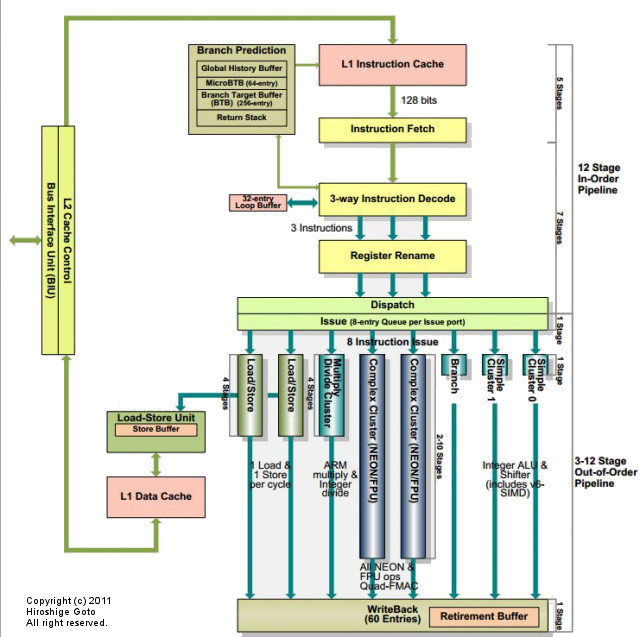
\includegraphics[width=1\textwidth]{img/Cortex_A15_Block_Diagram.jpg}
		\caption{Cortex A15 Block Diagram \cite{sloss2004arm}}
		\label{fig:blockdiagram}
	\end{figure}

	In our cache oriented obfuscation method, we have assumed the system which we worked on is Von Neumann so far. In our implementation, we showed deobfuscation code routine in listing\ref{code:obfuscation}. The reason why we can not simply implement this model is, it is working on the instruction section which actually stored in instruction cache, but in Modified Harvard architecture, there is no direct access to write instruction caches. As seen in figure \ref{fig:blockdiagram}, after fetching obfuscated instruction code into data cache and deobfuscation and storing it back to the cache, it does not move directly to instruction cache. It has to be evicted back to main memory and be fetched into instruction cache instead. Therefore, if we implement same code on Modified Harvard architecture, we encounter with incoherent cache issue which obstructs deobfuscation of instruction or we cause to leak our plain code to upper layer memory. If there is one more layer cache such as L2 cache, instruction and data cache communicate over those; however, it reduces our attack's stealthiness in any case.

\section{Solution}
	In brief and on the whole of mentioned issue in the previous section is the obstacles of modifying instruction cache's values. to sum up our issue, we have two caches which are "dcache" which we can read and write but can't not execute and "icache" which we can execute but can't read\footnote{we can't read it directly, but we can observe its results and estimate it.} and write, thereby we can not deobfuscated and run obfuscated code in the same cache. The question we answered in this section is whether it is possible to redesign a running program's control flow in support of data which it is working on or not. It is only possible, when we design instructions and  statements in the program depending on the branches, namely values that branches depending on. In computer science convention, some methods of interpretation is equivalent to our definition and requirement, and it is shoved that the ability of the interpreter can be equal to ability of the machine it is working on\cite{mak2011writing}\cite{abelson1996structure}. Even though it is possible to building our own interpreter, it is not recommended, because it will be embedded in "Icache" which is plain text and possible to identifying and obtaining signatures. Therefore, we propose to use well known interpreter; then, it could be legalized on signature detection phase.

	\subsection{Flying over Interpreter}
	Instead of running a machine code on target system, we proposes interpreting byte codes or structured abstraction (and therefore it is not bound to any specific machine code but the interpreter itself) for Harvard architecture system. It makes malware architecture independent(On the other hand, it is still cache dependent malware) except stub part. Although Interpretation and compilation are two different methods, they are tightly coupled terms in computer programming. Hence, they are not mutually exclusive on implementation of high level language. Interpreted or compiled languages mean the canonical implementation of the language is compiler or interpreter based\cite{mak2011writing}.

	There are typically several variants of interpreters in a spectrum between compiling and interpreting\cite{mak2011writing}. Byte code interpreting is a method for parsing code directly from interpreter language to byte code. The byte code is not machine code for specific architecture, but machine code for the interpreter's virtual machine. The byte code representation of the corresponding code is generally highly compressed and optimized because they uses all compilation techniques and backgrounds, but efficiency depending on the interpreter and architecture relationship\cite{mak2011writing}. The second variant of the interpreters is using intermediate representation of interpreter's source code. Concrete and abstract syntax tree interpreters are the two of the most known and acknowledged examples. It has more overhead than byte code representation, but it is easier to interpret and preform better analysis during runtime because of better structure and relation representation between statements of the code\cite{mak2011writing}. The one of another variant is just-in-time compilation. They are not pure interpreters or compilers. This techniques compile byte code or intermediate representation to the native code at runtime. Therefore, it is not appropriate for our methods to use because it is still compilation and running native code directly. 

	In figure \ref{fig:blockdiagram}, our approach is illustrated. In this example, there is one shared memory, one "Icache", one "Dcache" and one CPU. It is a part of the whole system, and we assume there are more nodes connected to the same shared memory, but only one of the nodes showed in figure. Stub section of the Icache inherited from the previous chapters. Basically, it deobfuscates body of the malware  which is stored in dcache. As we can load, process and store values to dcache, stub implementation and internals are same. However, when we need to run the deobfuscated code on dcache, we use interpreter to bypass the obstacle, in contrast to previous proposals. Feeding interpreter from memory has already been supported by most of the interpreters for embedded devices e.g. Python, Forth, Basic interpreters. The only thing they need generally starting address. In addition to previous proposals, after running body of the malware, obfuscation could be handled by interpreter at the end of the gadget, or a tail section must be added, after interpreter code in Icache. 
	


	\begin{figure}[h!]
	\centering
	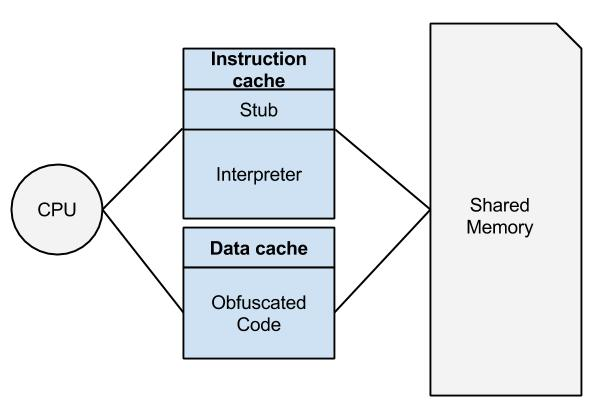
\includegraphics[width=1\textwidth]{img/Harvard_implementation.jpg}
	\caption{Illustration of Our Approach}
	\label{fig:blockdiagram}
	\end{figure}

	\subsection{Forth Interpreter Language}
		Forth programmers traditionally pay importance and emphases complete understanding and control over the machine and its architecture. Therefore, first principle of Forth is simplicity and openness, and it is completely documented and clearly easy designed. Koopman says in 1993 "Type checking, macro preprocessing, common subexpression elimination, and other traditional compiler services are feasible, but usually not included in Forth compilers and this simplicity allows Forth development systems to be small enough to fit in the on-chip ROM of an 8-bit microcontroller. On the other hand, Forth's extensibility allows "full-featured" systems to consume over 100K bytes and provide comprehensive window-based programming environments."\cite{koopman1993brief}, and it is more than fit for recent systems. This simplicity is one of the most important reason why we choose it for our implementation, but the most important reason, it gives you full control between compilation and interpretation. Beside, it is also designed for the embedded systems which use ROM memory instead of ICache, but similarly with our approach, it is read only memory, so it is treasury for our approach. 

		Because there is no explicit Forth parser and no formal grammar, it does not have many concrete standard. There are a few words with ANS Fort which are compiled in assembly, so it is quite simple and small. Moreover, Fort interpreter is very elastic to implement assembly words or remove them, but the standard forth interpreters are better options in term of stealthiness. 

		There are two level of interpretation in Forth, which are text and address interpreting\cite{koopman1993brief}. While text interpreting accepts keyboards or file inputs, address interpreting accepts memory inputs. Text interpreter mode parse white-space separate character string and determine their role in the process. First, it checks whether extracted string is word or not. if it is a word; then, do interpret word's statements, else it checks whether number or not. if it is number then push it to stack, else return exception. It is main control flow of the Forth text interpretation\cite{pelc2011programming}. On the other hand, address interpretation is a bit more complex. It used to execute Forth words which are actually dictionary structures. They all stitched each other with address pointers, and ultimately they point assembly word which is mentioned above and embedded in Forth interpreter. Therefore, there are a few root words which are written in assembly and children words which point parents and ultimately roots. 

\todo[inline]{Add an example code}
\section{Pitfalls and Fallacies}
	In this chapter, we do not concern the difficulties arise from cache coherency mechanism and we worked on incoherent caches. It is probable to implement "flying over interpreter" method with timing attack approach, but there is much more complexity on implementation phases. However, it theoretically has same principles. During implementation of stepped control flow, there could be more overhead related to interpretation. When we need to calculate interpretation latency, we should consider algorithmic overheads. The code which is processed by interpreters frequently uses threaded code. Threaded code refers to implementation of call routine and their consistence. We should also consider the latency which is arising out of this threaded code overhead, and prefer proper algorithms to decide interpreter. 

	Throughout this chapter, we never modified the values in instruction chapter, which is the head of our gadget and involve with an interpreter and stub parts. In order to prevent misunderstanding, it is better to underline that we can modify the values in the instruction cache, but if we move values from the data cache to instruction cache, it will lose its stealthiness, but not vice verse. Therefore, we can move instruction cache values in the data cache and modify them freely. It gives us an ability to regenerate stub part again and again.

	Abstract syntax tree method as an intermediate interpretation language is pretty compact and compressed representation of byte codes\cite{kistler1999tree}, but produce more overhead\cite{garen2008announcing}, so it is better to use it systems without cache coherency. Also, code density can vary from compilation method to method. Because we have limited space, it is better to fit as much as code in minimum space. Due to the division of data and instruction caches, Harvard systems have half sized cache for data.